%%
%% This document uses the Elsevier 'cas-dc' (Complex Article Service,
%% double-column) class, as required for Elsevier journal submissions.
%%
\documentclass[a4paper,fleqn]{cas-dc}

\usepackage[authoryear,longnamesfirst]{natbib}
\usepackage{amsmath,amssymb}
\usepackage{tikz}
\usetikzlibrary{shapes.geometric,arrows.meta,positioning,fit,backgrounds}

\begin{document}
\let\WriteBookmarks\relax
\def\floatpagepagefraction{1}
\def\textpagefraction{.001}

% Short title
\shorttitle{Non-Uniform Frost Detection Using Multi-ROI Visual Analysis}

% Short author list
\shortauthors{Shahryar et al.}

% Main title of the paper
\title[mode=title]{Computer Vision-Based Detection and Spatial Quantification of Non-Uniform Frost Accumulation on Evaporator Coils Using Multi-ROI Analysis}

% Title footnote
\tnotemark[1]
\tnotetext[1]{This research did not receive any specific grant from funding agencies in the public, commercial, or not-for-profit sectors.}

% First author
\author[1]{M. Shahryar}
\cormark[1]
\ead{shahryar@ceme.nust.edu.pk}
\credit{Conceptualization, Methodology, Writing -- original draft}

\affiliation[1]{organization={Department of Mechatronics Engineering, CEME, National University of Sciences and Technology (NUST)},
            addressline={},
            city={Islamabad},
            postcode={44000},
            state={},
            country={Pakistan}}

% Second author
\author[1]{M. Ibrahim}
\credit{Investigation, Software, Writing -- review \& editing}

% Third author
\author[1]{Seemal}
\credit{Data curation, Validation}

% Fourth author
\author[1]{Sarim}
\credit{Formal analysis, Writing -- review \& editing}

% Corresponding author text
\cortext[1]{Corresponding author}

% Abstract
\begin{abstract}
Frost accumulation on the evaporator coils of refrigeration systems severely degrades thermal performance, restricting airflow and significantly driving up power consumption. Traditional frost detection paradigms often simplify this issue by treating accumulation as a completely uniform layer or by relying on localized physical point sensors, thereby failing to capture the complex spatial variations across the coil geometry. To address this limitation, this paper presents a novel artificial intelligence-driven computer vision framework designed to detect and quantify non-uniform frost development. By establishing a comprehensive matrix of Regions of Interest (ROIs) across the entire surface of the evaporator coil, the proposed approach facilitates full-field spatial tracking. Utilizing tailored digital image processing and deep learning architectures, our system successfully quantifies frost thickness non-uniformity across both the horizontal and vertical spatial directions simultaneously. Experimental validation carried out on a domestic refrigeration platform demonstrates that this multi-ROI spatial profiling provides high-fidelity localized thickness mapping, offering a robust, data-driven foundation for next-generation, on-demand intelligent defrosting strategies.
\end{abstract}

% Research highlights
\begin{highlights}
\item A multi-ROI computer vision framework is proposed for non-uniform frost detection.
\item Frost thickness is quantified simultaneously along horizontal and vertical axes.
\item A pixel-to-physical calibration model converts segmented masks to frost thickness maps.
\item A non-uniformity index and per-ROI uncertainty estimation support localized defrost control.
\end{highlights}

% Keywords
\begin{keywords}
Frost detection \sep Frost thickness estimation \sep Computer vision \sep Artificial intelligence \sep Non-uniform frosting \sep Refrigeration automation
\end{keywords}

\maketitle

\section{Introduction}\label{sec:intro}
Frost formation on heat exchange units presents a pervasive and critical challenge in refrigeration and heat pump technologies, acting as an insulating thermal barrier that restricts volumetric airflow, diminishes cooling capacity, and elevates power consumption \citep{mehmood2025frost,wang2023eulerian}. To mitigate these adverse operational effects, timely detection and accurate frost thickness quantification are vital for orchestrating energy-efficient, on-demand defrosting cycles rather than relying on conventional, rigid timed schedules \citep{alcaraz2023virtual,chen2024utilizing}. In recent years, non-contact monitoring solutions leveraging computer vision and artificial intelligence have gained substantial traction due to their ability to replace degradation-prone physical sensors with high-fidelity, real-time visual diagnostics \citep{akbar2024deep,elahi2026transformer}. However, standard visual detection schemes predominantly analyze the evaporator coil as a single homogeneous entity or measure thickness at a single localized zone, neglecting the highly non-uniform spatial distribution of frost caused by localized microclimate fluctuations, humidity gradients, and refrigerant flow variations \citep{babadi2023localized}. To overcome this limitation, this study introduces an intelligent computer vision framework that strategically establishes multiple distributed Regions of Interest (ROIs) across the entire evaporator coil surface. The core novelty of this work lies in its capability to dynamically segment and quantify frost thickness non-uniformity along both horizontal and vertical spatial dimensions simultaneously. By mapping these multidirectional variations on individual evaporator rods, the proposed framework provides an exceptionally granular representation of localized frosting kinetics, effectively bridging a critical gap in the development of precise, localized defrost control strategies for modern sustainable refrigeration systems.

\section{Literature Review}\label{sec:litrev}
It is well-established that frost formation reduces refrigeration efficiency, resulting in lower heat transfer rates, increased compressor running times, and component wear and tear. Over time, ice accumulates on the entire evaporator surface, hindering airflow, increasing overall thermal resistance, and forcing the system to operate more to meet the desired cooling requirements. Most traditional defrost systems employ timed defrost cycles based on assumptions of uniform frost distribution, but in reality, ice deposits unevenly due to variations in airflow patterns, humidity levels, temperature, and evaporator geometry. Uneven frost deposition causes a decline in cooling capacity, the formation of local cold spots, and renders the defrosting process less efficient. Therefore, studying the spatial and positional characteristics of frost deposition is crucial. For years, traditional frost detection methods, such as physical hardware-based approaches like pressure difference switches, electrical resistance sensors, and thermal sensors, have been studied. While these methods can detect the presence of frost, they typically fail to provide spatial and geometric information about frost thickness across the evaporator. As a result, researchers are increasingly turning to computer vision (CV) and artificial intelligence (AI) to detect frost without physical contact and to determine local frost thickness.

Initial efforts in frost thickness detection focused on classifying whether frost had formed. More recently, research efforts have shifted towards estimating continuous frost thickness instead of simple classification. This is because early-stage frost deposits act as insulating layers on heat transfer surfaces, making it essential to measure frost thickness before it forms into solid ice. Numerous AI algorithms and image processing techniques have been applied by researchers to estimate frost thickness distribution on evaporator surfaces. For example, \citet{akbar2024deep} proposed a CNN-based approach for estimating frost thickness in domestic refrigeration units, achieving 98.10\% accuracy for frost thicknesses ranging from 0 to 4 mm. Similarly, \citet{rahman2023cloud} developed a cloud-based IoT frost monitoring system using ESP32-CAM and Sobel edge detection, achieving a frost thickness error of 10.8\%, which was superior to conventional photoelectric and k-means methods. However, their analysis of frost thickness was limited to a few locations on the evaporator and did not provide a frost distribution map of the entire evaporator. \citet{mehmood2025frost} developed a modified EfficientNet for frost estimation (Frost-EffNet) using Grad-CAM to improve model interpretability, achieving an MAE of 0.11 mm and 92.47\% classification accuracy, with the ability to identify regions that contributed to the model's predictions. Additionally, \citet{chen2024utilizing} utilized CNN to classify frost severity on evaporators using surveillance images, achieving 97.57\% accuracy, reducing defrost frequency and energy consumption. However, this system assigns a single frost class to the entire evaporator, preventing local frost analysis. To avoid hardware complexity, \citet{andrade2025acoustic} proposed an inexpensive and easy-to-implement acoustic-based frost detection system using a speaker and microphone with ANNs and PNNs models, achieving 94\% classification accuracy. Nonetheless, this technology does not provide information on frost deposition location. \citet{alcaraz2023virtual} developed a virtual frost sensor using refrigerator temperature data and an RF classifier, achieving 73\% accuracy without any physical hardware frost sensor. The system reduced unnecessary defrost cycles, resulting in improved energy efficiency, but it could not differentiate spatial variations in frost formation. Recent research focuses on modeling non-uniform and localized frost deposition on refrigerators. \citet{babadi2023localized} analyzed localized frost deposition using both CFD simulations and experiments on an LG refrigerator, demonstrating higher frost deposition near the return duct rather than uniformly, and showing that reducing the number of fins could decrease local frost thickness by approximately 13\%. In a similar vein, \citet{wang2023eulerian} developed a Eulerian two-phase CFD model for predicting frost growth on circular tubes, reporting average errors of 6.0\% for thickness prediction and 8.1\% for frost density, and observed rapid frost accumulation on windward surfaces under reduced air velocity.

Using computer vision, \citet{aguiar2023local} addressed the issue of local frost detection on heat exchangers, optimizing sensor coverage by 21.4\% and reducing blind spot error by 16.8\%. The same authors \citep{rahman2024sobel} employed Sobel edge detection with k-means to extract point-wise frost thickness on evaporator surfaces, achieving a prediction error and RMSE of 13.69\% and 0.19 mm, respectively. \citet{elahi2026transformer} utilized a transformer-based semantic segmentation model to obtain pixel-wise frost thickness distribution, achieving an $R^2$ of 0.93 and an IoU of 0.875, along with 93\% accuracy on their dataset. \citet{han2023comparison} compared various machine learning models (ANN, SVM, Ridge, and LASSO) for frost thickness prediction in refrigerators, with the ANN model achieving 94.2\% accuracy and an RMSE of 0.16 mm. Distributed sensing technologies, such as capacitance-based sensing proposed by \citet{shen2023capacitance}, can measure frost distribution on heat exchangers with an accuracy of 0.1 mm but are generally impractical for domestic applications due to cost and complexity.

The current literature highlights extensive research efforts in AI, CV, and sensing technologies for frost detection and prediction. However, most existing approaches either classify overall frost presence or provide frost thickness estimates at limited localized points on the evaporator without accurately capturing the real-time full spatial distribution of frost, particularly under non-uniform frost conditions in domestic refrigeration systems. Based on the literature review, there is a significant demand for a low-cost, high-accuracy, and computationally efficient system capable of real-time, comprehensive monitoring of frost thickness distribution across the entire evaporator surface, especially when frost deposition is non-uniform. Current systems face challenges such as incomplete spatial coverage, dependence on costly and complex hardware, or focus only on general frost severity rather than detailed spatial variations. Our proposed work aims to bridge these gaps by developing a computer vision-based approach that uses an RGB camera to detect and quantify non-uniform frost deposition on individual evaporator rods. This system will provide continuous measurements of frost thickness both horizontally and vertically, along with uncertainty estimation, enabling highly accurate and adaptive defrost scheduling for refrigeration systems.

\section{Methodology}\label{sec:methodology}
The proposed framework uses a fixed-position RGB camera to monitor the evaporator coil of a domestic refrigeration unit [REFRIGERATOR MODEL] under controlled ambient conditions. Rather than treating the coil as a single homogeneous surface, the coil is discretized into a matrix of $m \times n$ Regions of Interest (ROIs) [SPECIFY GRID SIZE] spanning both the horizontal and vertical extent of the evaporator rods, with camera position, focal length, and illumination held constant to ensure consistent image acquisition throughout each frost accumulation cycle.

Each captured frame is preprocessed through geometric calibration, illumination normalization, and noise reduction, then cropped into the predefined ROI matrix. Frost boundaries within each ROI are segmented using [SPECIFY METHOD: CNN-based segmentation / edge detection / transformer-based segmentation], and local frost thickness is estimated from the segmented mask using [SPECIFY: regression head / geometric mask analysis]. Pixel-based measurements are converted to physical thickness using a calibration factor $k$ (mm/pixel), obtained from known-dimension reference markers in the camera's field of view:
\begin{equation}\label{eq:calib}
T_{i,j} = k \cdot P_{i,j}.
\end{equation}

The resulting ROI-wise thickness values are assembled into a two-dimensional frost thickness map. Horizontal and vertical profiles are extracted by averaging $T_{i,j}$ along each axis, and a non-uniformity index (coefficient of variation of $T_{i,j}$) quantifies overall spatial unevenness at each time step. Per-ROI measurement uncertainty is estimated by repeating acquisition over $N$ independent trials under identical conditions and computing the standard deviation of the resulting estimates.

Model performance is validated against manually annotated ground-truth measurements using MAE, RMSE, $R^2$, and IoU, computed both globally and per-ROI to assess overall accuracy as well as consistency across spatial locations on the evaporator surface.

\subsection{Flowchart}\label{sec:flowchart}
Fig.~\ref{fig:flowchart} summarizes the end-to-end methodology described above, from image acquisition through ROI-wise frost thickness estimation to spatial mapping and validation.

\begin{figure*}[t]
\centering
\resizebox{0.72\textwidth}{!}{%
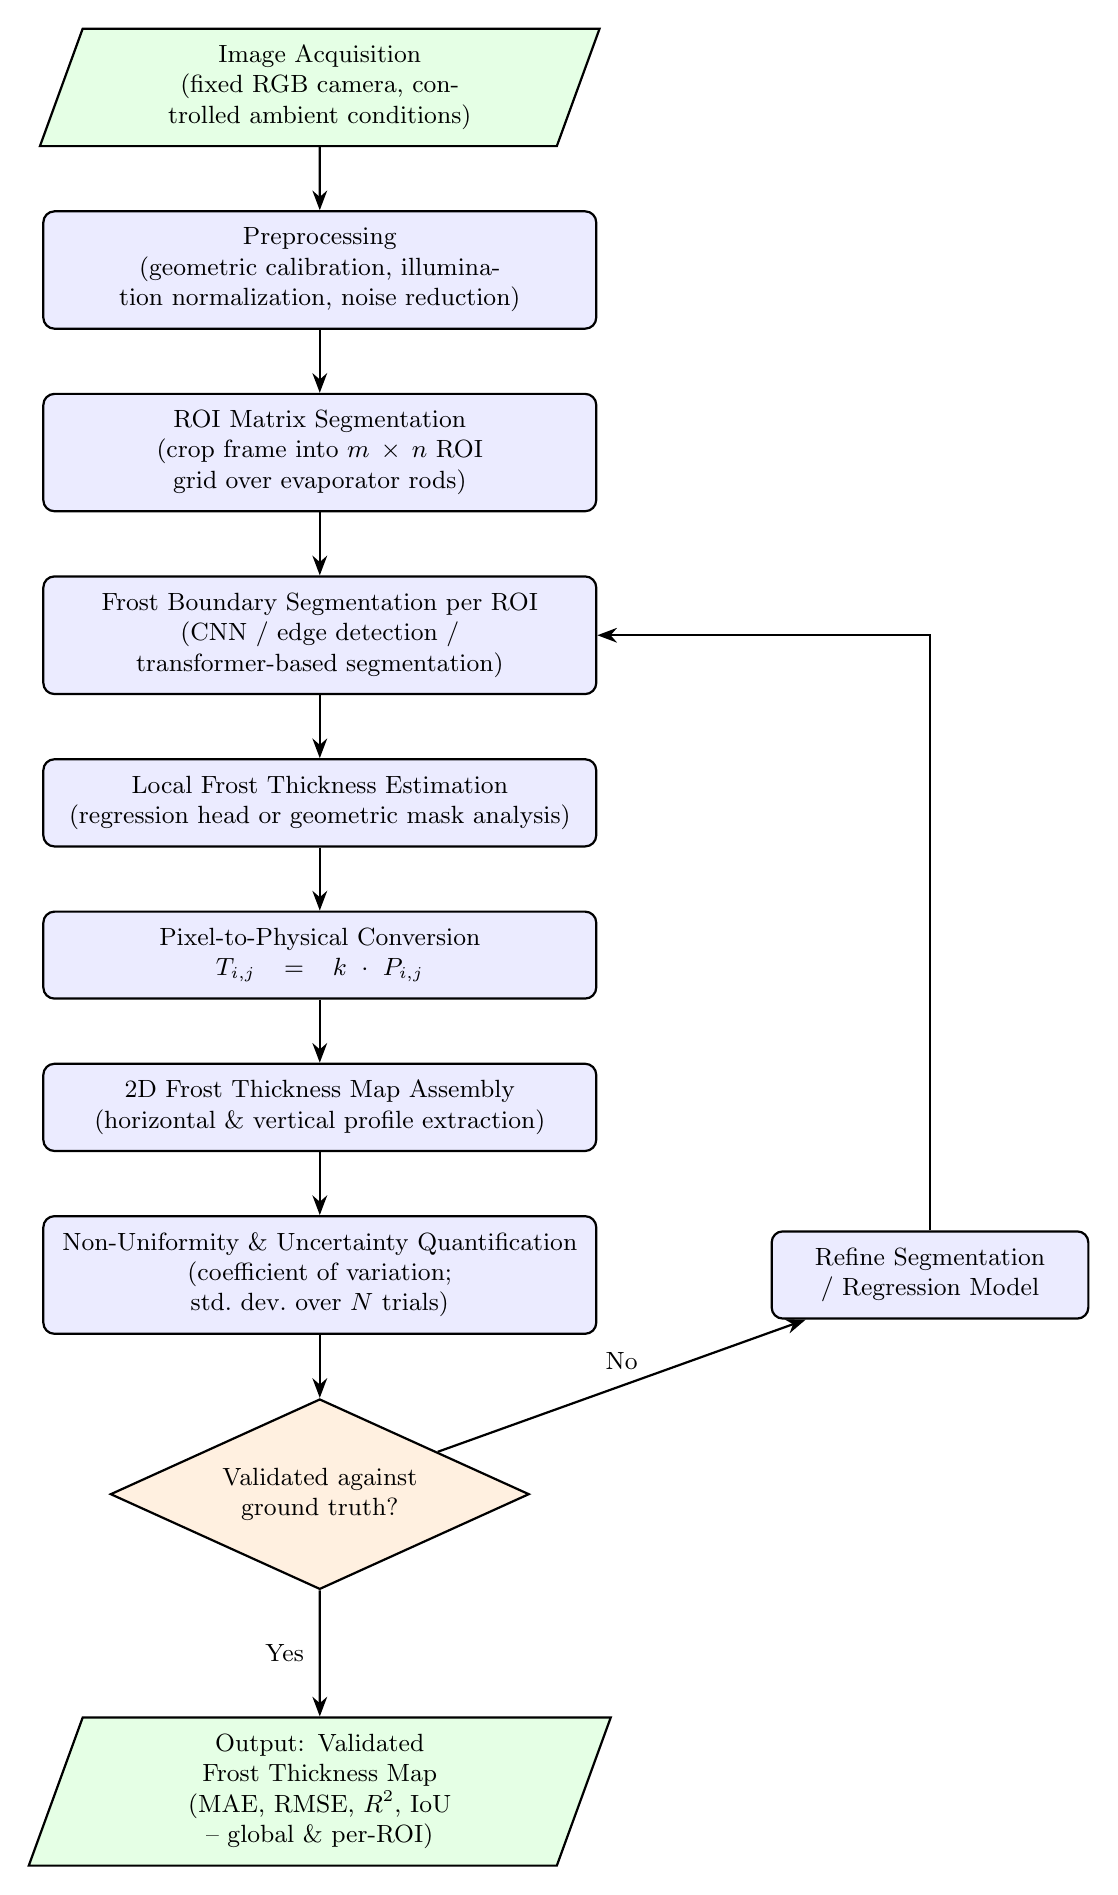
\begin{tikzpicture}[
  node distance=0.8cm and 1.2cm,
  font=\small,
  process/.style={rectangle, rounded corners, draw=black, thick, fill=blue!8,
                  text width=6.6cm, minimum height=1cm, align=center, inner sep=6pt},
  decision/.style={diamond, draw=black, thick, fill=orange!12,
                   text width=3.4cm, minimum height=1.1cm, align=center, inner sep=2pt, aspect=2.2},
  io/.style={trapezium, draw=black, thick, fill=green!10, trapezium left angle=70,
             trapezium right angle=110, text width=5.6cm, minimum height=1cm, align=center, inner sep=6pt},
  arr/.style={-{Stealth[length=2.5mm]}, thick}
]

\node[io] (acq) {Image Acquisition\\(fixed RGB camera, controlled ambient conditions)};
\node[process, below=of acq] (pre) {Preprocessing\\(geometric calibration, illumination normalization, noise reduction)};
\node[process, below=of pre] (roi) {ROI Matrix Segmentation\\(crop frame into $m \times n$ ROI grid over evaporator rods)};
\node[process, below=of roi] (seg) {Frost Boundary Segmentation per ROI\\(CNN / edge detection / transformer-based segmentation)};
\node[process, below=of seg] (thick) {Local Frost Thickness Estimation\\(regression head or geometric mask analysis)};
\node[process, below=of thick] (calib) {Pixel-to-Physical Conversion\\$T_{i,j} = k \cdot P_{i,j}$};
\node[process, below=of calib] (map) {2D Frost Thickness Map Assembly\\(horizontal \& vertical profile extraction)};
\node[process, below=of map] (nu) {Non-Uniformity \& Uncertainty Quantification\\(coefficient of variation; std.\ dev.\ over $N$ trials)};
\node[decision, below=of nu] (valid) {Validated against\\ground truth?};
\node[io, below=1.6cm of valid, text width=5.6cm] (out) {Output: Validated Frost Thickness Map\\(MAE, RMSE, $R^2$, IoU -- global \& per-ROI)};
\node[process, right=2.2cm of nu, text width=3.6cm] (refine) {Refine Segmentation / Regression Model};

\draw[arr] (acq) -- (pre);
\draw[arr] (pre) -- (roi);
\draw[arr] (roi) -- (seg);
\draw[arr] (seg) -- (thick);
\draw[arr] (thick) -- (calib);
\draw[arr] (calib) -- (map);
\draw[arr] (map) -- (nu);
\draw[arr] (nu) -- (valid);
\draw[arr] (valid) -- node[left, xshift=-2pt] {Yes} (out);
\draw[arr] (valid) -- node[above, yshift=2pt] {No} (refine);
\draw[arr] (refine) |- (seg.east);

\end{tikzpicture}%
}
\caption{Flowchart of the proposed multi-ROI computer vision methodology for non-uniform frost thickness detection and spatial quantification on evaporator coils.}
\label{fig:flowchart}
\end{figure*}

% To print the credit authorship contribution details
\printcredits

%% Loading bibliography style file
\bibliographystyle{cas-model2-names}

% Loading bibliography database
\bibliography{references}

\end{document}